% !TEX root = ../master-thesis.tex


\begin{figure}[h]
    \centering
    \addletter{90}{a}
    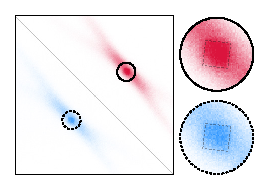
\includegraphics{fig-ai/loading-from-odt-1-ai.pdf}
    \phantom{42}
    \addletter{90}{b}
    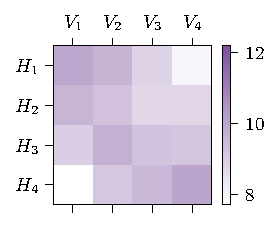
\includegraphics{fig-py/loading-from-odt-2.pdf}
    \phantom{42}
    \addletter{90}{c}
    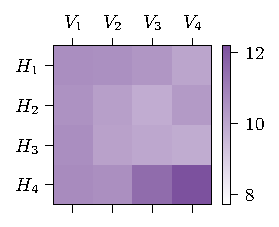
\includegraphics{fig-py/loading-from-odt-3.pdf}
    \caption{
    \textbf{Inhomogeneous loading from ODT to tweezer arrays.}
    (a) Atom distribution for a $6\times6$ array (averaged over 10 realizations), demonstrating inhomogeneous loading from the optical dipole trap (ODT).
    (b) Observed atom number distribution for a uniformly powered $4\times4$ tweezer array, revealing systematically lower loading efficiency at corners (averaged over 30 realizations).
    (c) Improved uniformity after manual adjustment of tweezer intensities, specifically enhancing corner powers (averaged over 30 realizations).
    }
    \label{fig:loading-from-odt}
\end{figure}
